\documentclass{article}
\usepackage{style-assessments}

% define macros (/shortcuts)

\begin{document}

\hspace{375pt}Name:

\begin{center}
{\Huge MATH 321: Review Part 3}

\end{center}

\bigskip\bigskip

% problem types summary
% 1) paired t-interval and interpretation
% 2) one prop Z-test and interval
% 3) one mean t-test (RR) and interval
% 4) regression diagnostics
% 5) R regression application


\begin{enumerate}
    \item The University is investigating the safety of MATH courses for their students. To do this, they plan a study to compare the blood pressure of upper level MATH courses students before the final exam and after completing the final exam. Data are shown below (in mm Hg).% CSCC UPDATED LU 9 - Inferences from Dependent Samples
    \item[] Construct and interpret a 95\% confidence interval for the difference in blood pressure before and after the final exam for math students. State a conclusion if final exams increased blood pressure on average.
    \begin{figure}[H]
        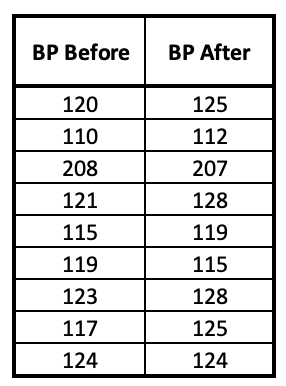
\includegraphics[scale=0.5]{images/data-bp.png}
    \end{figure}\vspace{100pt}
        
    \item The campus bookstore is determining if they need to increase their marketing budget. They would like at least 65\% of students to buy their textbooks directly from them rather than off-campus stores. In order to check this, they took a random sample of 137 students in which 81 students said they buy their books at the campus bookstore.% CSCC UPDATED LU 8 - Hypothesis Testing Overview and for Proportions
    \begin{enumerate}
        \item Is there enough evidence to conclude the true proportion of students who buy their books at the campus bookstore is greater than 65\%? Use $\alpha = 0.05$.\vspace{200pt}
        \item Construct the corresponding 90\% (two-sided) confidence interval. State a conclusion if this proportion is greater at least the desired 65\%.\vspace{100pt}
    \end{enumerate}
   

    \item Scientists discovered a new mountain range under the sea. Lets assume the sea mountain heights are normally distributed with unknown standard deviation.
    \item[] From a random sample of 13 peaks, there was an average height of 11,308 ft and standard deviation of 5,287 ft.% UPDATED LU 8 - Hypothesis Testing for Means All Days
        \begin{enumerate}
        \item Is there enough evidence to conclude the average heights of these new sea mountains is different than the Rocky Mountains, which average 14,400 ft? Use $\alpha = 0.12$.\vspace{250pt}
        \item Construct the corresponding (two-sided) confidence interval for this test and confirm your conclusion from part (a).\vspace{100pt}
    \end{enumerate}\newpage
    
    \item Given the following residual plots for the regression of $Y \sim X$, assess the assumptions of the normal error regression model.
    \begin{figure}[H]
        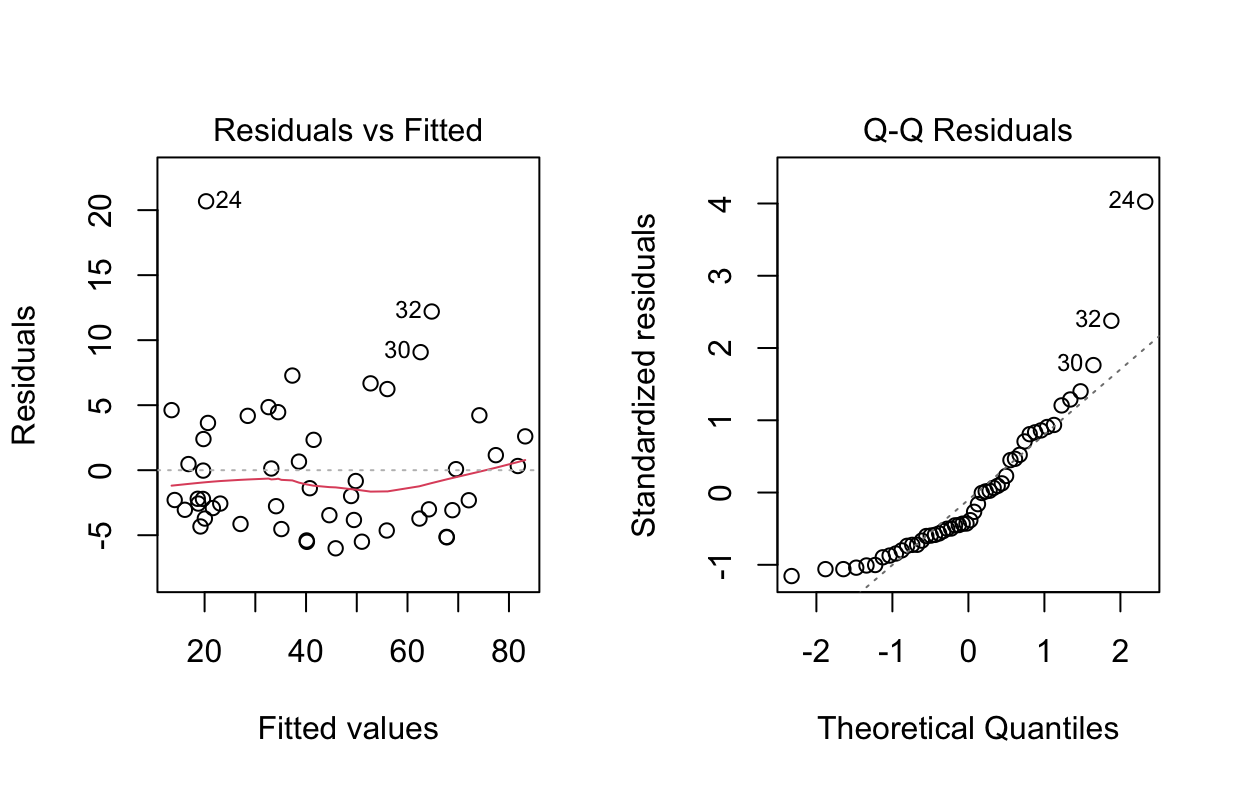
\includegraphics[scale=0.25]{images/non-normal-errors.png}
    \end{figure}\vspace{100pt}
    
    \item (Extra R practice, NOT ON FINAL) 
    \begin{enumerate}
        \item Using the data from question 1, perform EDA for the regression on After as the response variable and Before as the explanatory variable. Is there anything we should be concerned about beforehand?\vspace{150pt}
        \item Fit the regression from part (a) and get the estimated coefficients.\vspace{50pt}\newpage
        \item Perform a t-test on the slope coefficient. Use $\alpha = 0.01$\vspace{230pt}
        \item Predict the after blood pressure for a student with a before blood pressure of 123.\vspace{50pt}
    \end{enumerate}
        
\end{enumerate}

\end{document}